
\begin{figure}[h!]
    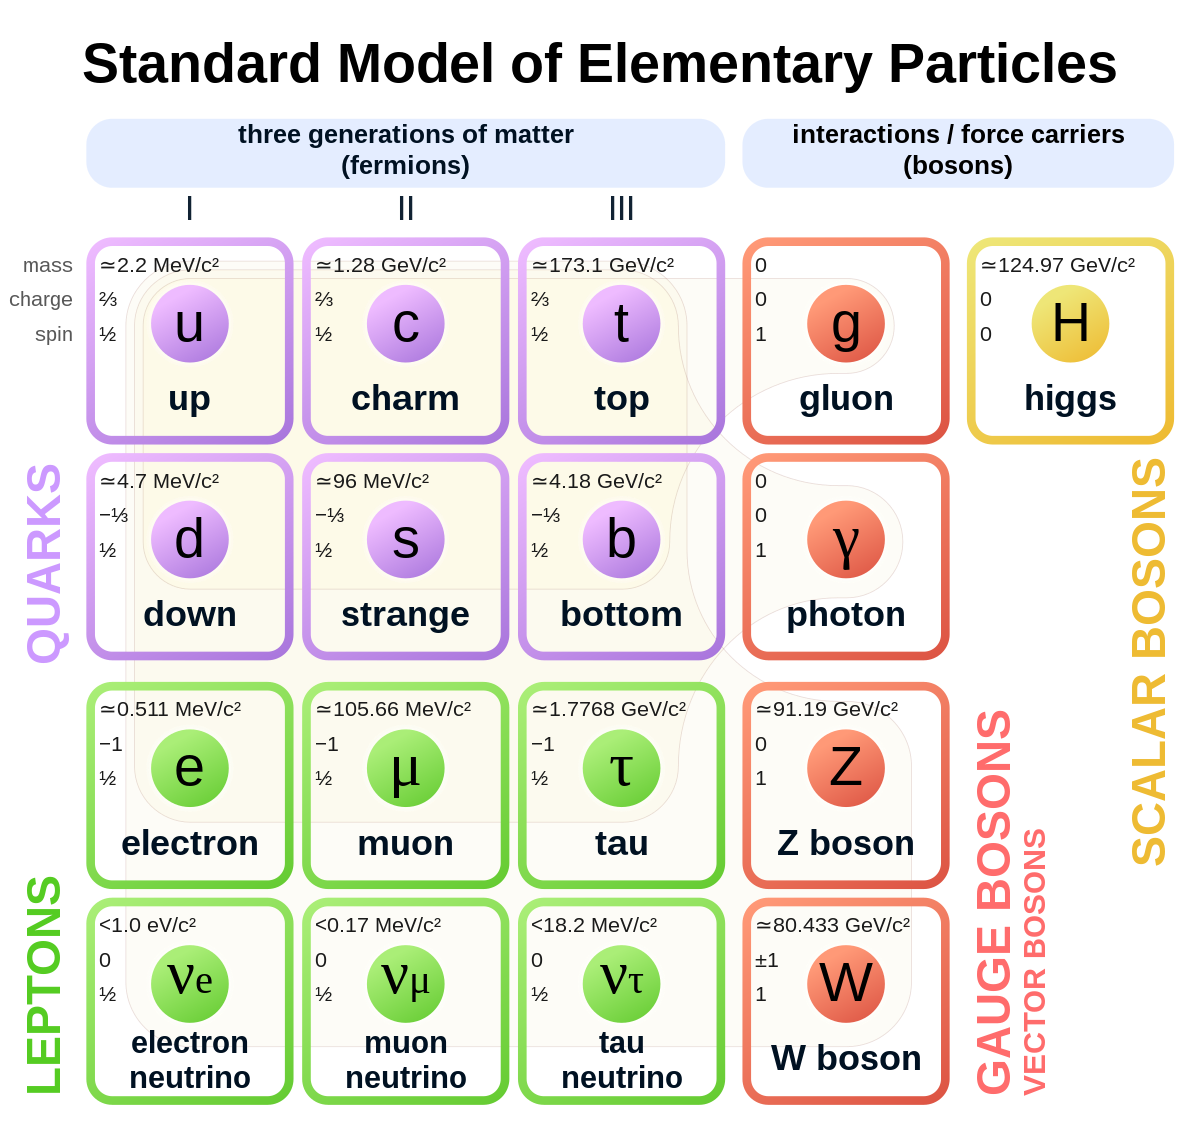
\includegraphics[width=\linewidth]{Figures/SM/Standard_Model_of_Elementary_Particles.svg.png}
    \caption{The standard model of elementary particles. Source \href{https://upload.wikimedia.org/wikipedia/commons/thumb/0/00/Standard_Model_of_Elementary_Particles.svg/1200px-Standard_Model_of_Elementary_Particles.svg.png}{here}. Accessed 07.10.22}
    \label{fig:smdiagram}
\end{figure}

\section*{Structure and composition of the Standard Model}
This section will describe the standard model in a phenomelogical way, as the mathematics and physical reasoning behind the theory is not of great 
importance to understand the work, nor the results or discussion of them. For a more technical explanation, read (Pich, 2008)\cite{Pich:819632} for a 
well written paper containing the some more standard model fundamentals, as well as summarizing the experimental status regarding the standard model.
For more mathematical understanding of the standard model, Peskin and Schroeder's "An introduction to Quantum Field theory" (Peskin and Schroeder, 1995)\cite{Peskin:1995ev}
 is highly recommended. Finally, for more understanding of particle physics, the nature of interactions and more, see Thomson's "Modern Particle physics" (Thomson, 2013)\cite{Thomson:2013zua}. \par


The standard model is to physicists what the periodic table is to chemists. It is comprised of two parent class particles, fermions and bosons, where fermions 
are comprised of quarks and leptons. The model contains 17 particles, 6 quarks, 6 leptons and 5 bosons, and are shown in figure \ref{fig:smdiagram}.



\subsection*{Fermions}
The fermions are the building blocks of matter, and contain two types of particles, leptons and quarks. Together they form protons and neutrons,  atoms all around us.
Fermions, unlike bosons, are spin half particles, and are also the only particles to have anti particles. The fermions are grouped into three so called families:
\begin{equation*}
    \begin{bmatrix}
        \nu_e & u \\
        e^{-} & d^{\, '} 
    \end{bmatrix},\quad
    \begin{bmatrix}
        \nu_{\mu} & c \\
        \mu^{-} & s^{\, '}
    \end{bmatrix},\quad
    \begin{bmatrix}
        \nu_{\tau} & t \\
        \tau^{-} & b^{\, '}
    \end{bmatrix}
\end{equation*}
Here, the first family consists of the electron, the electron neutrino, the up and down quarks. The second family consists of the muon and the
muon neutrino, the charm and strange quarks. The third family consists of the tau and the tau neutrino, the top and bottom quarks. The masses of these particles 
increases for each particle in the matrix as the family number increases, i.e the muon is heavier than the electron, and the tau is heavier than the muon, and so 
on for the other fermions. \par
Quarks are fractional charge particles, with defined charge of either $2/3$ or $-1/3$. They are the "main" building blocks of protons and neutrons, and are bound by the strong 
force, the strongest of the four fundamental forces. The force mediator is the gluon. The other fermions are leptons. They are split into the charged leptons (electrons, muons and taus),
and the uncharged leptons (neutrinos). The charged leptons can interact via the electroweak force, where the Z, W bosons as well as the photon can be a mediator.


\subsection*{Bosons}



\section*{Limitations}
All though the standard model have had great success comparing with experiments,
there are still several problems not addressed by it. First and foremost, the standard model
as described above, does not and cannot explain gravity in a quantized way. There 
are models that try to address this problem, but they supplement the standard model,
and does not derrive it from it. 



